\documentclass{article}
\usepackage[utf8]{inputenc}

\title{Project Two: Hill Climbing, Hill Climbing with Random Restarts, and Simulated Annealing}
\author{Gene Burchette}
\date{March 19, 2016}

\usepackage{natbib}
\usepackage{graphicx}

\begin{document}

\maketitle

\section{Introduction}
    Optimizing functions involves finding the global minimum or maximum of a given utility function, usually named the \textit{fitness function}. For this project, we focused on minimizing the given function (1).
    
    \begin{equation}
        z = \frac{sin(x^2 + 3y^2)}{0.1 + r^2} + (x^2 + 5y^2)\frac{exp(1 - r^2)}{2}, r = \sqrt{x^2 + y^2}
    \end{equation}
    
    
    \begin{figure}[hb!]
        \centering
        \includegraphics[scale=1]{surface.jpg}
        \caption{Graph of given function}
        \label{fig:surface}
    \end{figure}

    Some optimization methods like \textit{hill climbing}, the process of continually choosing a neighboring node with a higher fitness until a hill is reached, are quick at finding local maxima. As search spaces get more complex and have more jagged surfaces, hill climbing will get stuck on local minima, failing more often than succeeding when finding global minimum. An improvement to this algorithm is to continually hill climbing but restarting at random places in the search space and comparing cached local minima. This algorithm is named \textit{hill climbing with random restarts}. Again, as search spaces get even more complex and even discontinuous, the function will continually get trapped in local minima or result in undefined behavior. Another alternative is the \textit{simulated annealing} algorithm. This third algorithm accepts moving to a node with a less than ideal fitness value in hopes of getting unstuck from the local minima. This accepting process is determined by the equation (2).
    
    \begin{equation}
        P_{accepting\,bad\,state\,from\,A \to B} = e^\frac{f(B) - f(A)}{T}
    \end{equation}

    Once a potentially bad move is accepted, the algorithm will unstick itself and explore other local minima and again compared with cached local minima to estimate the global minima. One strong advantage about simulated annealing is that \textbf{a solution is \textit{guaranteed} so long as the temperature is lowered slowly enough.} Consequently, the slower T is lowered, the more costly this algorithm becomes in time expenditure.
    
    \clearpage
    
\section{Hill Climbing}
    During this project hill climbing was very successful at finding a local minima quickly. However, the purpose in optimizations is not to find a good solution, but rather to find the best solution. The downfall of hill climbing was once the algorithm reached a hill, all neighboring nodes would have a higher Z value, registering as a minimum and terminating the search. If this search space only had one minimum, hill climbing would be the best algorithm to use. However, the surface represented by equation (1) was more complex with multiple hills and valleys, seen in Figure \ref{fig:surface}. Conclusively, this algorithm was very poor at finding the global minimum on average, but very fast.
    
    \begin{figure}[hb!]
        \centering
        \includegraphics[scale=1]{hill_climbing.jpg}
        \caption{Hill Climbing}
        \label{fig:hillclimbing}
    \end{figure}
    
    \clearpage

\section{Hill Climbing with Random Restarts}
    Where hill climbing accepted a good solution as a terminating condition, hill climbing with random restarts only terminated once N hill climbing searches had been executed. When N = 1, Hill climbing with random restarts is exactly hill climbing (one iteration is actually no restarts). As the number of restarts increased, computation became more expensive and many times the same local minima was found over and over resulting in efficient searches. However, this algorithm was able to successfully find the actual global min many times with good timing as well (1-3 seconds). 
    
    \begin{figure}[hb!]
        \centering
        \includegraphics[scale=1]{hill_climbing_restarts.jpg}
        \caption{Hill Climbing with Random Restarts}
        \label{fig:hillclimbingrestarts}
    \end{figure}
    
    \clearpage

\section{Simulated Annealing}

    Simulate annealing was the slowest of the three algorithms when trying to make it actually calculate the global min but actually quite fast at getting very close to the global min (within .0001) in a very short time. I was unsuccessful in ever calculating the actual global min for this function with simulated annealing before computational overflow ensued. Compared to hill climbing with random restarts, hill climbing with restarts would very quickly find the actual min making simulated annealing seem inferior. Compared to hill climbing, this algorithm would not get stuck on local minima as easily and exceeded far better in getting close to the global min.
    
    \begin{figure}[hb!]
        \centering
        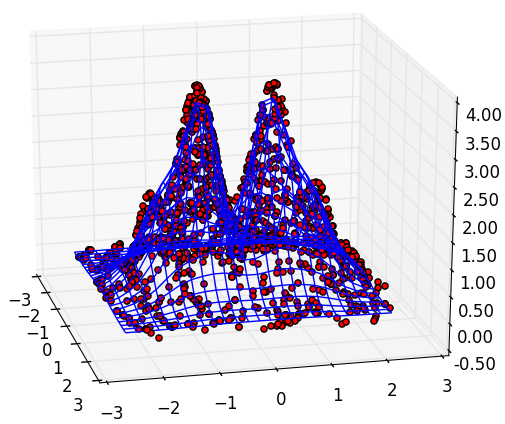
\includegraphics[scale=1]{simulated_annealing.jpg}
        \caption{Simulated Annealing}
        \label{fig:simulatedannealing}
    \end{figure}
    
    \clearpage

\end{document}